\section{Descrizione del sistema}
Il sistema è composto da varie pagine JSP ognuna delle quali fornisce uno specifico servizio al cliente. Ogni webpage include la tecnologia Javascript che consente non solo di migliorare l’interfaccia stessa della pagine ma permette anche di ottimizzare la facilità di navigazione.\\[1\baselineskip]Per sviluppare il sistema sono stati usati i seguenti tool:
\begin{itemize}
\item Adobe DreamWeaver CS5.5 per creare l’interfaccia grafica;
\item Eclipse Juno, per creare la logica di business;
\item Mysql Workbench, per visualizzare la base di dati.
\end{itemize}

\vspace{1.2cm}

\subsection{L'architettura del sistema}

SWIMv2 è sviluppato secondo l'architettura client-server, e quest'ultimo secondo il pattern MVC, in modo da tenere nettamente separati lo stato del sistema, la logica di
business e l'interfaccia grafica. In particolare, per quanto riguarda il client, possiamo immaginare che esso sia un comunissimo browser che manda delle richieste ad un server ed
elabora le sue risposte, mostrando all'utente le informazioni desiderate tramite la view. Il server invece è locale, ospita il database e la logica di business e fornisce un'interfaccia grafica personalizzata a seconda dello stato del sistema; tale stato varia a seconda dei comandi ricevuti dal
client, ma non in modo arbitrario: il controller si occupa di mantenere il DB in uno stato consistente e di comporre volta per volta il codice JSP da passare al browser; a questo proposito,
particolare importanza hanno le servlet, componenti che appunto generano le pagine web dinamiche che l'utente vede. Il server, come già specificato è JBoss AS 5, un'implementazione
open source della piattaforma J2EE.
\\

Possiamo riassumere la struttura dell' applicazione come una multi-tier composta dai seguenti livelli:
\begin{itemize}
\item Client tier: è composta dal client side dell’applicazione: si occupa di inviare le richieste al webserver tramite il browser. Include il codice Javascript e il codice JSP per la presentazione dei servizi.
\item Web tier: Hanno il compito di gestire la sessione con gli utenti del sistema e di ricevere da quest’ultimi gli input inviati e di passarli quindi al business tier.
\item Business tier: gestisce la logica di sistema
\item Data tier: comprende la base di dati della quale si servirà il business tier. Tale base dati comprenderà tutti i dati e tutte le informazioni del sistema.
\end{itemize}

\begin{figure}
\centering
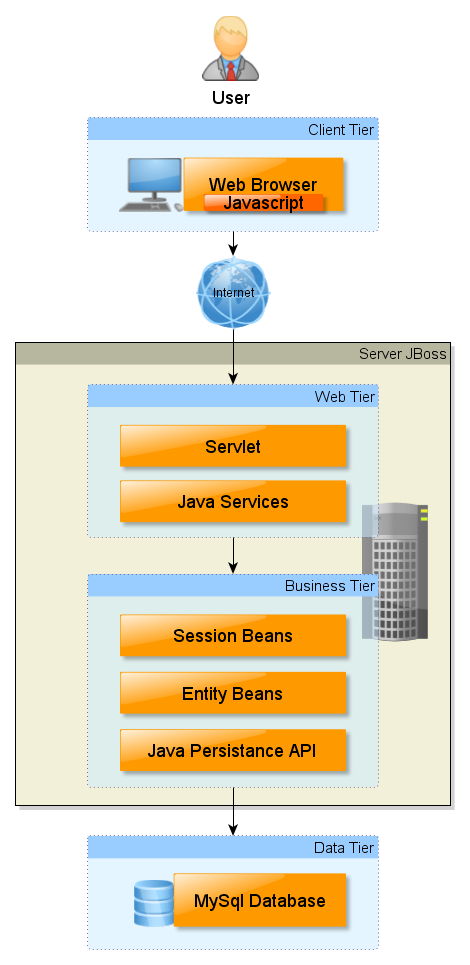
\includegraphics[scale=0.6]{tierdesign.png}
\caption{\label{architettura} Architettura e schema di deployment del sistema}
\end{figure}

\subsection{Scomposizione in sottosistemi}

L'applicazione si può suddividere in sistemi componenti, un' analisi legata alla gestione delle funzioni principali di SWIM ci ha portato ad individuare: il login, i sottosistemi di ospite, utente registrato, amministratore e l’archiviazione dei messaggi, discussioni, registrazioni ecc.
\begin{itemize}
\item Login: si occupa della gestione dell’accesso al sistema, in base alla tipologia dell’utente seleziona il sottosistema di utilizzo; 
\item Archivio: si occupa della memorizzazione dei dati importanti per le attività all'interno della piattaforma quali la memorizzazione dell'utenza registrata e dei contenuti tramite l'utilizzo del DBMS ; 
\item Ospite: interagisce col sistema tenendo conto delle restrizioni imposte dallo stato anonimo dell’utente (impossibilità di replicare ai messaggi, inviare feedback…)
\item Utente registrato: gestisce tutte le azioni dell’utente autenticato e la condivisione delle informazioni del suo profilo
\item Amministratore: gestisce sia tutte azioni esclusive dell’amministratore (come l’accettazione di nuove abilità) che quelle comuni all’utente registrato (come l’invio di messaggi)
\end{itemize}

L’esistenza dei sottosistemi dell’utenza di SWIM è giustificata dalla loro diversa interazione con l’archivio.\\[1\baselineskip]Gli amministratori potranno modificare le tabelle all’interno del DBMS, gli utenti registrati interagiranno con l’archiviazione dei messaggi e infine gli ospiti potranno visualizzare il contenuto di una parte dei dati senza poter apportare nessuna modifica; è bene precisare che le funzionalità di tali sottosistemi non sono in mutua esclusione infatti la ricerca all'interno dell'applicazione può essere svolta da tutti gli internauti. \\[1\baselineskip]Per gestire tale meccanismo abbiamo scelto una soluzione che prevede di sfruttare la logica dell’applicazione, essa sarà in un certo senso intelligente e secondo l’appartenenza di classe renderà possibili le corrispettive interazioni con il database; ciò eviterà inutili accessi all'archivio.

\clearpage

\begin{figure}
\centering
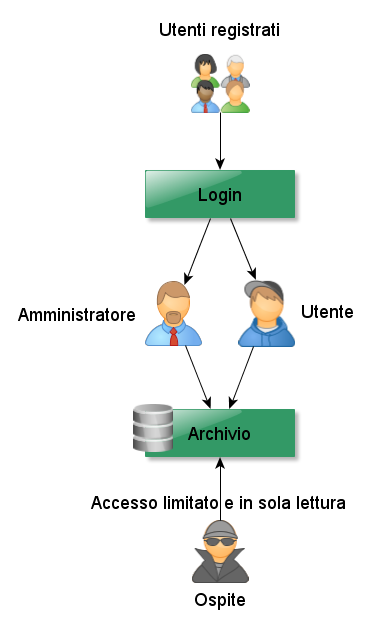
\includegraphics[scale=0.8]{sottosistemi.png}
\caption{\label{sottosistemi} Rappresentazione dei sottosistemi e delle loro interazioni}
\end{figure}

\pagebreak